%===================================== CHAP 5 =================================

\chapter{Analysis}

\todo[inline]{Make a table with baseline classification rate for logistic regression, put in our values. 1 Peer with no noise, 1 peer with noise, best case from other experiments that we want to highlight. This can lead to a discussion of why our results are not as good, where they show promise etc}

All prediction results given in this section are presented with mean and standard deviation values. These values are computed by evaluating each combination of parameters with 10-fold cross validation and taking the mean and standard deviation of accuracy across the 10 data folds.

As explained in section \ref{section:differential_privacy}, differential privacy works by disguising an individual's data in a dataset by adding noise to their records. The amount of noise added is determined by the privacy parameter  $\epsilon$, and grows exponentially the closer the parameter gets to zero. 

\begin{figure}[H]
	\centering
	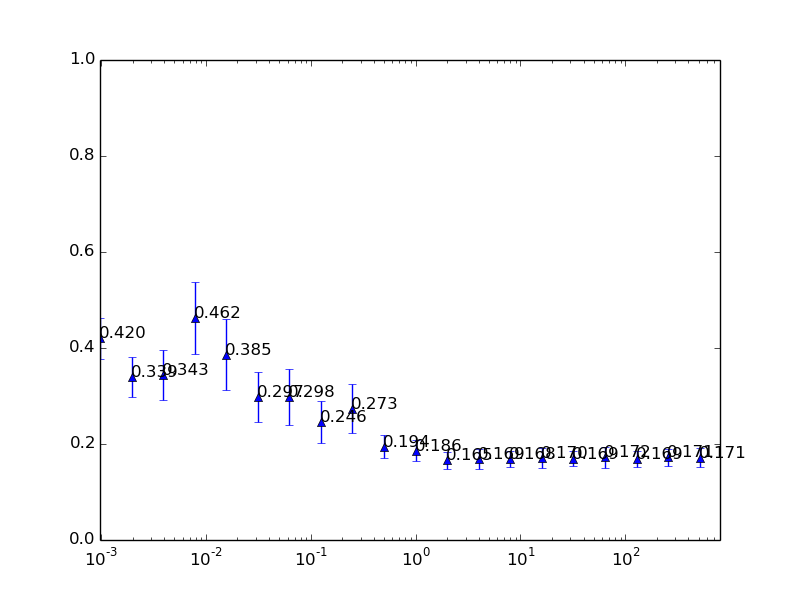
\includegraphics[width=\textwidth]{fig/eps2e-10-2e9,bud=eps,peers50,groups50,reg2e-4}
 	\caption{$\epsilon = [10^{-3}, 10^{3}], \lambda = 2^{-4}$, 50 peers, 1 aggregation}
 	\label{fig:epsilon_big_range}
\end{figure}
 
Figure \ref{fig:epsilon_big_range} shows the effect of the privacy parameter $\epsilon$ in our experiment. We wanted to test the effect of varying the $\epsilon$-value in the range from $2^{-10}$ to $2^9$, especially to find out how the classifier would perform when faced with data with high amount of noise added to it. The positive class rate in the UCI Spambase dataset is 0.4, so any error rate at this level is no better than a random classifier. The plot shows how sensitive output is to the values of $\epsilon$

Figure \ref{fig:linear_epsilon_range} 

\section{The importance of data}
One of the more important findings for 
Data is important, the more data a peer have, the greater the chance is that it will make a decent local classifier. J

\begin{figure}[H]
	\centering
	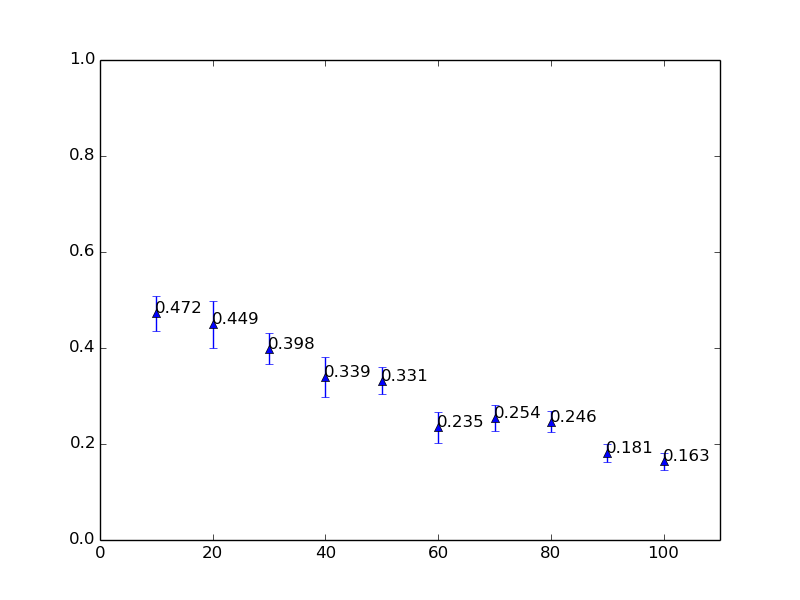
\includegraphics[width=\textwidth]{fig/eps0.3,budg=eps,peers30,groups5,reg2e-2-pubAll-datalimitTEST}
	\caption{$\epsilon = [0.3], \lambda = 2^{-2}$, 30 peers, 1 aggregation}
	\label{fig:data_limit_test}
\end{figure}




\begin{figure}[h!]
	\centering
	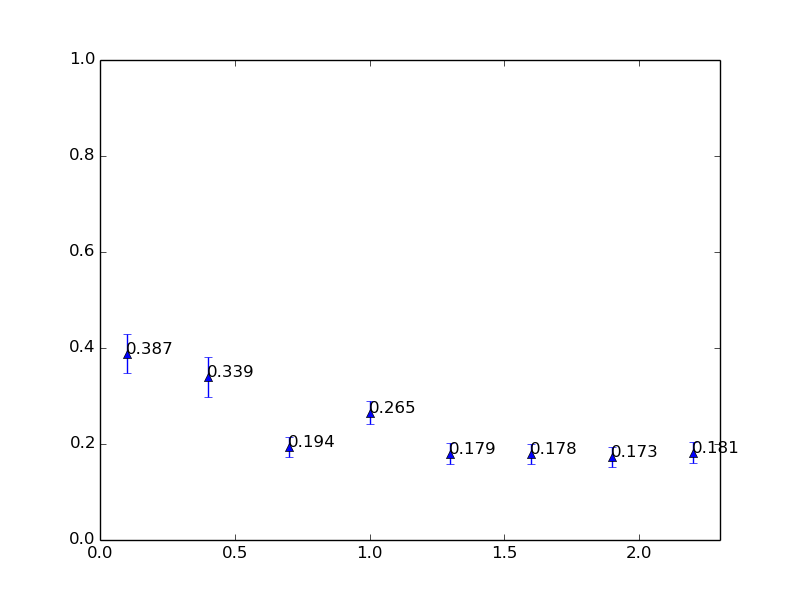
\includegraphics[width=\textwidth]{fig/eps0.1-2.2,bud=eps,peers50,groups50,reg2e-4}
	\caption{$\epsilon = [0.1, 2.2], \lambda = 2^{-4}$, 50 peers, 1 aggregation}
	\label{fig:linear_epsilon_range}
\end{figure}

\begin{figure}[h!]
	\centering
	\begin{minipage}{.49\linewidth}
		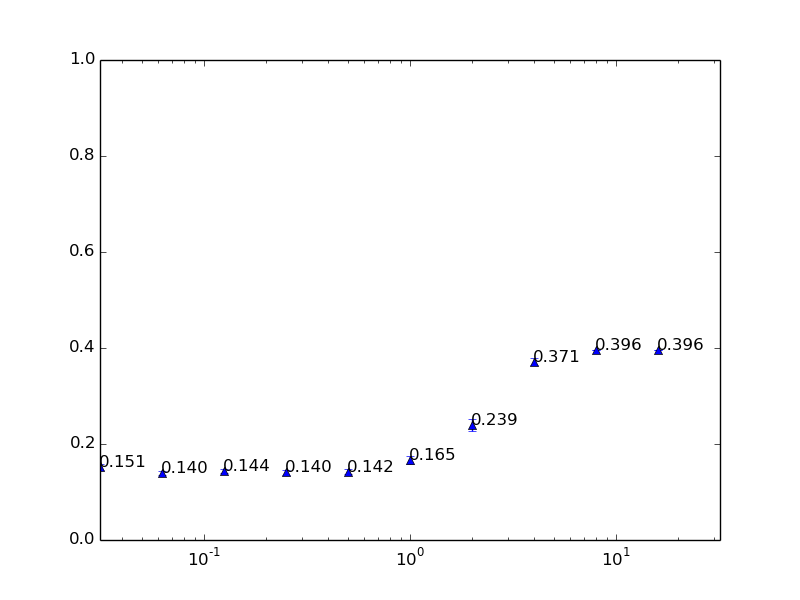
\includegraphics[width=\linewidth]{fig/spambase/eps2e10,budg=eps,peers50,groups2,reg2e-5-2e4-pubAll-LRbyCV-retuning}
		\captionof{figure}{$\epsilon = 2^{10}, \lambda = [2^{-5}, 2^{4}]$, 50 peers, 25 aggregations, publish to participants}
		\label{fig:regularization_normalepsilon}
	\end{minipage}
	\hspace{.001\linewidth}
	\begin{minipage}{.49\linewidth}
		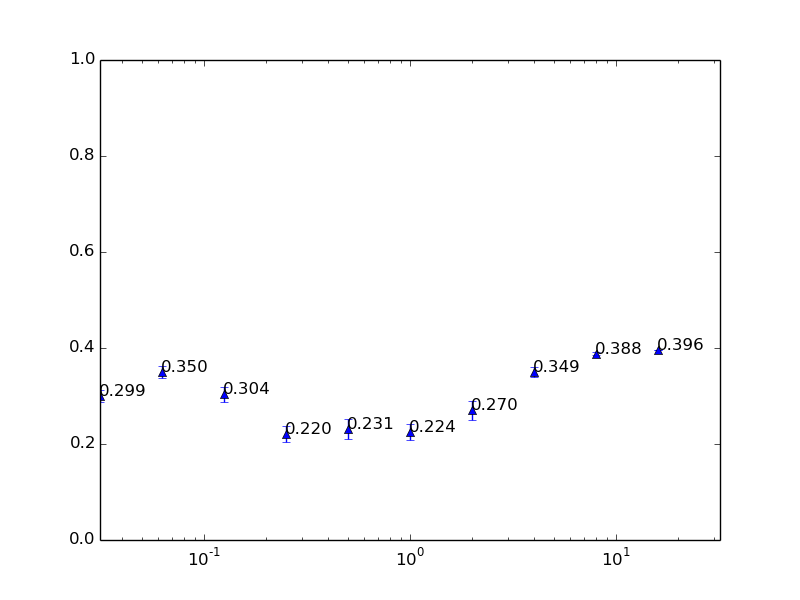
\includegraphics[width=\linewidth]{fig/spambase/eps0.1,budg=eps,peers50,groups2,reg2e-5-2e4-pubAll-LRbyCV-retuning}
		\captionof{figure}{$\epsilon = 0.1, \lambda = [2^{-5}, 2^{4}]$ 50 peers, 25 aggregations, publish to all}
		\label{fig:regularization_extremelyhighepsilon}
	\end{minipage}
\end{figure}

Figure \ref{fig:regularization_extremelyhighepsilon} shows the normal effect regularization has on accuracy for the spambase data set, by setting $\epsilon$ so high that noise is essentially nonexistent. As the regularization parameter $\lambda$ grows large, the model becomes less able to fit the training data, eventually resulting in models predicting only the negative class, which constitutes 60\% of the data set. This happen because the high regularization forces the parameter vector to the zero vector, resulting in uniform class probability for all samples. 

On this particular dataset it appears that a logistic regression model is not at risk of overfitting, since the cross validated error does not increase when the level of regularization is very low. Ignoring the effects of privacy mechanisms, this would mean that selecting some regularization parameter in the range $[10^{-5},10^{-2}]$ could be acceptable. Choosing a level at the high end of this range could be a good idea, to reduce the risk of overfitting.


Figure \ref{fig:regularization_normalepsilon} shows mean accuracy over a range of $\lambda$ similar to Figure \ref{fig:regularization_extremelyhighepsilon}, where $\epsilon$ is set to a level where the noise variance still has an effect on prediction accuracy, as seen in figure \ref{fig:epsilon_big_range}.

When noise with significant variance is added to the model creation process, tuning $\lambda$ will adjust noise variance as well. Equation \ref{eq:aggregated_logistic_sensitivity} states that the noise variance is inversely proportional to $\lambda$. The choice of regularization then must balance the model flexibility at lower levels of $\lambda$ with the decreased noise at higher levels of lambda.


\subsection{Analysis of Propagation and group size}

As mentioned in Section \ref{sec:PropagationPubModel}, we hypothesized that we could improve the overall classification accuracy of our system by publishing the aggregated models generated in phase 2.\unsure{Rewrite this if we don't use phases} 

\begin{figure}[h!]
	\centering
	\begin{minipage}{.49\linewidth}
		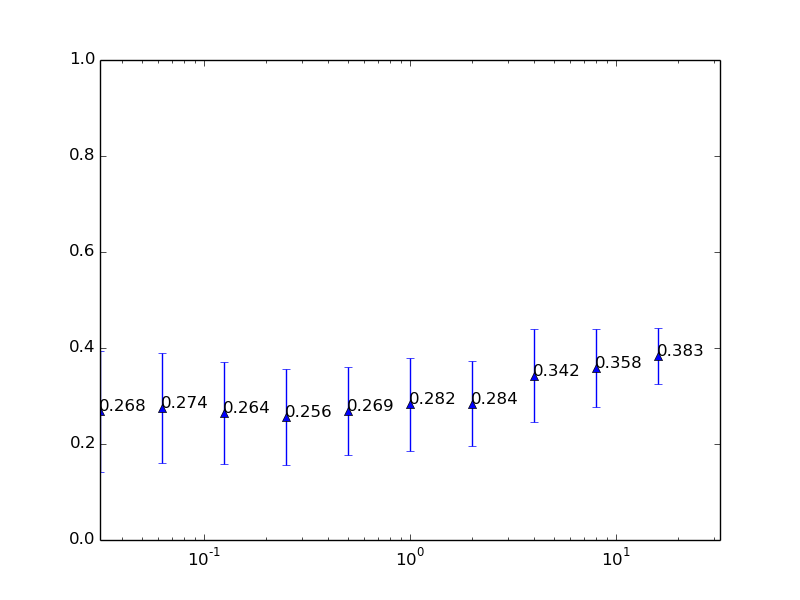
\includegraphics[width=\linewidth]{fig/PartyAllComparisonSpam-eps1.0,budg=eps,peers50,groups2,reg2e-5-2e4-pubParty-LRbyCV-retuning.png}
		\captionof{figure}{$\epsilon = 1.0, \lambda = [2^{-5}, 2^{4}]$ 50 peers, 25 aggregations, publish to participants}
		\label{fig:RegRangeTestPubParty}
	\end{minipage}
	\hspace{.001\linewidth}
	\begin{minipage}{.49\linewidth}
		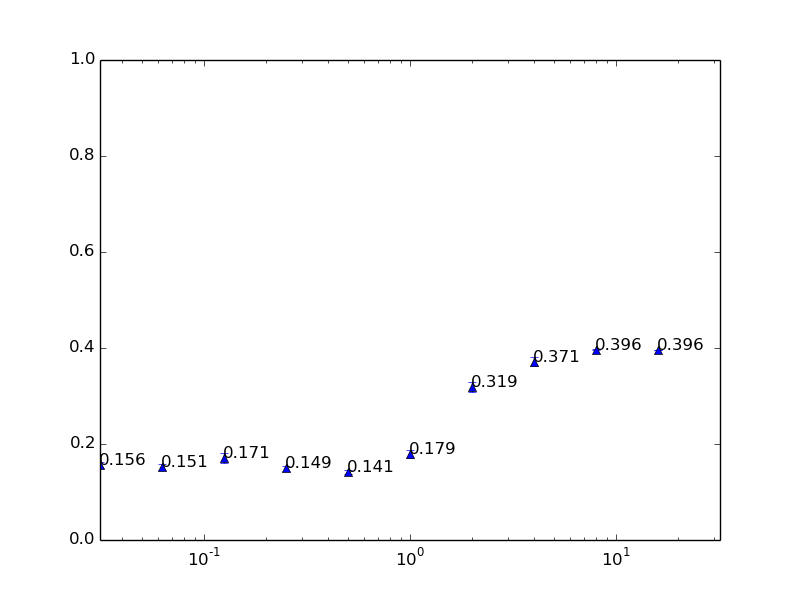
\includegraphics[width=\linewidth]{fig/PartyAllComparisonSpam-eps1.0,budg=eps,peers50,groups2,reg2e-5-2e4-pubAll-LRbyCV-retuning.png}
		\captionof{figure}{$\epsilon = 1.0, \lambda = [2^{-5}, 2^{4}]$ 50 peers, 25 aggregations, publish to all}
		\label{fig:RegRangeTestPubAll}
	\end{minipage}
\end{figure}

As the previous experiment indicates that publishing newly made models to as many peers as possible is better \todo{Add a reflection talking about why this makes sense.}, we performed an additional experiment to determine whether it in such a scenario would be better to perform many aggregations with fewer models included in each aggregate or performing few aggregations including many models. This was achieved by testing performance with a range of values. In the experiment, each peer can only participate in a single aggregation before reaching the limit set by the privacy guarantee. For example, given a set of 50 peers, a aggregation size of 25 can only publish two aggregated models.
 
\begin{figure}[h!]
	\centering
	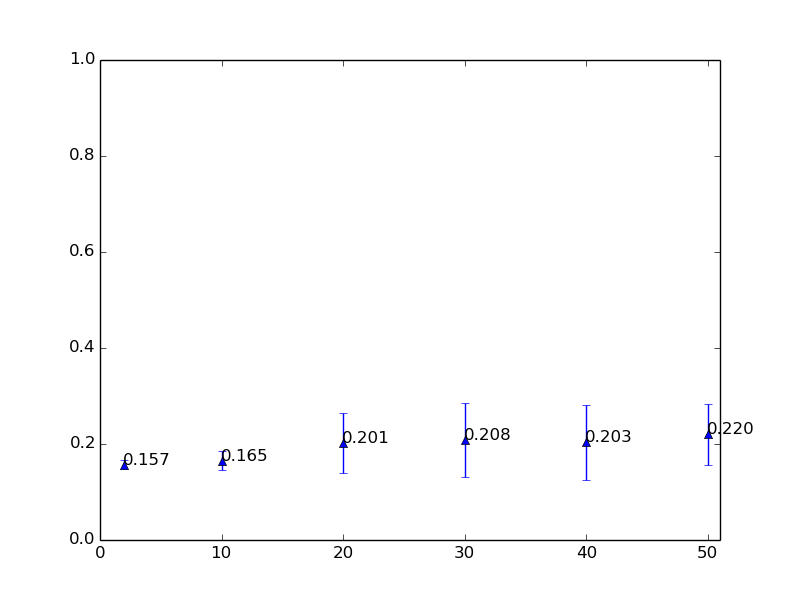
\includegraphics[width=\textwidth]{fig/GroupSizeEffectSpam-eps1.0,budg=eps,peers50,groups2-50,reg2e0-pubAll-LRbyCV-retuning}
	\caption{Spambase. $\epsilon = 1.0, \lambda = [1.0]$, 50 peers, aggregation sizes in range [2, 50], 66 samples per peer}
	\label{fig:groupsize_is_better}
\end{figure}

The results of this experiment is seen in Figure \ref{fig:groupsize_is_better}. It is clear that a smaller group size and consequently more aggregated models published resulted in a strong reduction in accuracy variance. While the variance is too high at larger group sizes to know much about the actual mean value after only 10 repetitions of the experiment, it is unlikely that it is smaller than the mean accuracy observed when the group size is one. 

A possible explanation of this result is that the effects of boosting counters the loss in accuracy that results from the addition of noise. Since models will have noise added to them before being published, expending all data to produce a single model might yield a worse classifier than partitioning data, adding noise to each separate, weaker model and combining them in an ensemble. On the other hand, this effect could be caused by some leakage of privacy which becomes visible over repeated applications of the aggregation mechanism. \todo{Figure out if there is some way we could test or prove that this is not the case.} 

The interesting observation that can be made from this is that the best situation is when there is no aggregation. A group size of one results in only a single model being contributed, and is equivalent to each peer publishing its local model with noise. One possible reason for this could be that there simply is no value in averaging models in the way done in our experiments and by Pathak et al.\cite{pathak2010diffprivhomo}. Neither our experiment or the experiment by Pathak et al. help distinguish between these two possibilities. The experiment by Pathak et al. only demonstrate that their method for creating aggregated models has comparable performance to adding noise to a centrally computed model. Additionally, this is only demonstrated with large data sets. In their experiment, the minimum data set size for any participant is 3256. With data sets this large, it is possible they would have gotten similar results by testing a model produced by a single participant, without performing additional aggregation. However, no experiment evaluating this possibility remains. Their theoretical conclusions stand, but experimentally validating the value of aggregation is necessary.

\todo{look at a couple of vectors trained with large subsets of data and see if they are similar.} Thus the key question is whether or not aggregation is worth the complexity of a homomorphic encryption protocol. If similar performance can be achieved solely by ensemble classifiers of differentially private models published by each peer, one could skip the complexity and risk of relying on a cryptographic protocol to maintain privacy.

Another possible explanation for this observation is that aggregation might be useful, but not when the peers all have samples of data from the exact same distribution. This is the case with the Spambase data set used in the experiment in Figure \ref{fig:groupsize_is_better}.

One way to answer question would be by finding a data set which has subsets that are produced by distinct distributions, and partitioning data by source distribution. Due to time constraints we did not have time to locate and prepare data sets that fit this requirement. \todo{See if we have time to do this. We REALLY sho1uld, otherwise it will very possibly give a lower grade.}

An alternative avenue for validating the value of doing aggregation could be to reduce the amount of data given to each peer. If just one peer has data sufficient to train a good classifier, it is sufficient. For that reason it makes sense to stage a situation were it is highly unlikely that even a single peer gets a lucky subset of data. Figure \ref{fig:groupsize_limiteddata} demonstrates such a case.

\begin{figure}[h!]
	\centering
	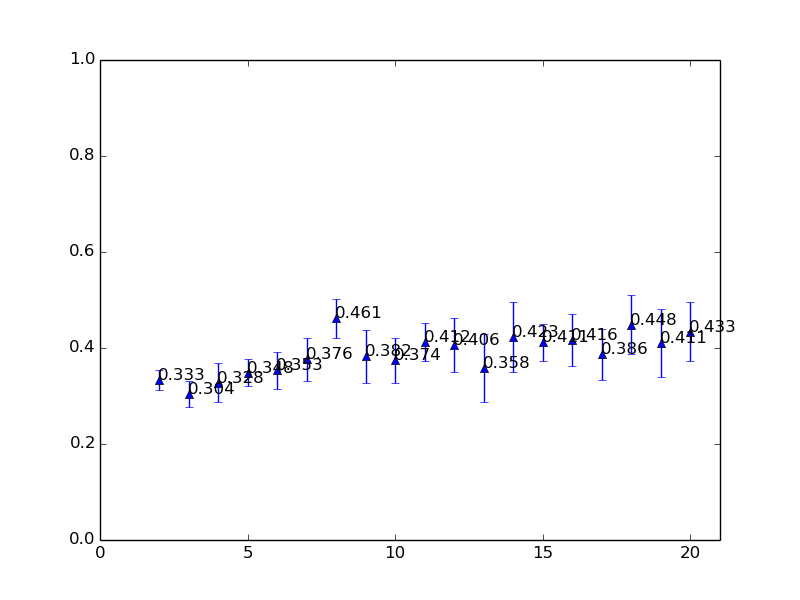
\includegraphics[width=\textwidth]{fig/spambase/ShowingPotentialUsefulnessOfLargerGroups-eps1.0,budg=eps,peers50,groups2-20,reg2e-2-dataMax20-pubAll-LRbyCV-retuning}
	\caption{Spambase. $\epsilon = 1.0, \lambda = [1.0]$, 50 peers, aggregation sizes in range [2, 50], 20 samples per peer}
	\label{fig:groupsize_limiteddata}
\end{figure}
\todo[inline]{redo this experiment above with regularization=0, as indicated by the previous figures shown}

What are the results of our experiments?

What did we learn from the basic structure of creating our framework?

What difficulties did we encounter?

What can we take away from our experiments?

What should have been done better? 

What did we learn from tuning the different parameters?

More data per peer leads to better classification. With small number of peers, there are more records per peer. This generally leads to better classification accuracy. Why is this? 

Australian: Sweet spot for regularization at a 2e-3, 10 peers 5 groupsize

What was the effect of tuning the regularization parameter? High and low regularization leads to more SD on the error rate, but there is a sweet spot.

What was the effect of increasing the epsilon? 
	It seemed like it was better to keep the perUpdateBudget smaller than the epsilon, so that the models are aggregated more. Did this lead to better accuracy? Why do more aggregations lead to better classification than having a bigger budget but only one aggregation.
	
Compare the results of our distributed logistic regression classifier with the tradional ones in literature. Sharma and Arora \cite{sharma2013adaptive} report getting 92.95\% classification accuracy on the same data set. Kumar et al\cite{kumar2012comparative}. reports  0.1389 error rate before filtering when using logistic regression combined with a least squares regularization method. Our classifier can compare to these under certain circumstances, even after noise addition.  



\section{Potential Future applications}
This section will discuss the potential application of a system based on our distributed machine learner.

\subsection{Health}
A growing worldwide market is the sale and usage of wearable sensors, such as environmental sensors, motion sensors, and health sensors. A IHS report \cite{ihs2014reportwearables} from 2014 estimates that the market for sensors in wearables will expand to 135 million units in 2019, up from 50 million in 2013. These wearables will evolve from being just a single purpose device such as a pedometer and grow into more multipurpose devices such as a smartwatch, which will consist of several sensors which can monitor several components within its area of use. 

The wearable devices are implementing fitness and health monitoring by using a mixture of sensors, such as motion, pulse, hydration and skin temperature sensors. All of these wearables will therefore generate a massive amount of data about the person who are using them. This data can be considered as highly sensitive information, as it can unveil a lot about their user's health, and the manufacturers of these devices knows this. Dana Liebelson, a reporter for Huffington Post, queried several US-based fitness device companies about their privacy. One of the replies she got, was that "the company does not sell information collected from the device that can identify individual users", but that they were considering marketing aggregate information that cannot be linked back to an individual. As we saw in section \ref{section:privacy_breaches} and \ref{section:attack_vectors}, many of the popular methods for aggregating and anonymizing a dataset carries an inherent risk of a privacy breach.

This is where we see a potential application for our distributed framework, as it solves the problem faced by those who don't want to give up control of their data to a third party, but they still want to analyze their data as it can be highly useful. 

-Future homes can potentially track you through you phone, or similar device. 

-You don't want to send this data to someone else, but what you can learn from the data can be highly useful in your daily life if analyzed. 

Kevin Fong and the England rugby team. Monitor heart rate, step balance, and a lot of other factors. Can pick up injuries and illnesses well before any doctor. This will trickle down into daily use over the next decade, and let people potentially discover illnesses before they even occur. 


\cleardoublepage